\chapter{Pengembangan \textit{Dataset Trace} I/O NFS dengan Beban Kerja Pelatihan Pembelajaran Mendalam}

\section{Analisis Permasalahan}
Dalam tugas akhir ini terdapat empat permasalahan utama. Pertama, penentuan format dan struktur \textit{dataset trace} I/O NFS. Kedua, pengembangan \textit{tracer} yang digunakan untuk mengembangkan \textit{dataset trace} I/O NFS selama beban pelatihan pembelajaran mendalam dijalankan. Ketiga, pengumpulan dan/atau pengembangan beban kerja pelatihan pembelajaran mendalam yang representatif. Keempat, pelaksanaan analisis terhadap karakteristik I/O yang dihasilkan oleh berbagai strategi \textit{shuffling} (\textit{global, buffered}, dan \textit{bundle}).


\subsection{Penentuan Format dan Struktur \textit{Dataset Trace} I/O NFS}
Dalam pengembangan \textit{dataset trace} I/O NFS, langkah awal yang krusial adalah mengidentifikasi jenis informasi yang perlu direkam. Pemahaman terhadap informasi ini akan menentukan desain dan mekanisme \textit{tracer} yang dikembangkan, khususnya bagaimana \textit{tracer} tersebut mencatat aktivitas I/O selama proses pelatihan model pembelajaran mendalam. Informasi yang dikumpulkan harus mampu merepresentasikan pola akses I/O NFS secara akurat serta relevan untuk mendukung analisis dan pengembangan sistem \textit{cache} dan \textit{prefetching} yang lebih efisien.

Setelah menentukan jenis informasi yang di-\textit{trace}, langkah berikutnya adalah menentukan format \textit{dataset trace} I/O NFS yang dikembangkan. Format tersebut harus memungkinkan peneliti untuk dengan cepat memahami, mengolah, dan mengintegrasikan data \textit{trace} ke dalam berbagai eksperimen atau sistem simulasi mereka. Kemudahan dalam pengembangan dan penggunaan \textit{dataset} sangat penting agar dapat mendukung keberlanjutan riset di bidang \textit{caching} dan \textit{prefetching}.


\subsection{Pengembangan \textit{Tracer}}
Untuk menghasilkan \textit{dataset trace} I/O NFS, perlu dikembangkan sebuah \textit{tracer} yang mampu merekam aktivitas I/O secara spesifik selama beban kerja pelatihan pembelajaran mendalam berlangsung. Prioritas utama dalam pengembangan \textit{tracer} ini adalah integritas data, yang mencakup keakuratan dan kelengkapan informasi yang ditangkap. Meskipun demikian, aspek efisiensi dan \textit{overhead} minimal juga menjadi pertimbangan krusial untuk memastikan proses \textit{tracing} tidak menganggu atau mengubah perilaku asli dari beban kerja pelatihan yang sedang diamati.


\subsection{Beban Kerja Pembelajaran Mendalam}
Langkah awal dalam perancangan beban kerja adalah menentukan jenis tugas pembelajaran mendalam, karena setiap tugas (misalnya, klasifikasi gambar atau deteksi objek) memiliki karakteristik I/O yang unik. Untuk menciptakan skenario yang relevan dengan tantangan komputasi modern, beban kerja dirancang dengan dua karakteristik kunci. Pertama, digunakan \textit{dataset} berukuran besar yang mampu menciptakan I/O \textit{bottleneck} pada lingkungan komputasi umum dengan sumber daya terbatas, seperti Google Colab, di mana keterbatasan memori memaksa sistem untuk terus bergantung pada penyimpanan. Kedua, data diakses secara berulang melalui pelatihan \textit{multi-epoch}, yang merupakan skenario ideal untuk mengukur efektivitas sebuah \textit{cache} melalui \textit{hit ratio}. Kombinasi inilah yang secara konsisten menghasilkan beban kerja terikat I/O: kondisi di mana performa sistem tidak lagi dibatasi oleh kecepatan komputasi, melainkan oleh latensi akses data.

\subsection{Analisis Karakteristik I/O NFS}
Karakteristik I/O pada beban kerja pelatihan pembelajaran mendalam cenderung berbeda dibandingkan dengan aplikasi umum lainnya \parencite{360survey}. Proses pelatihan biasanya melibatkan pembacaan \textit{dataset} berukuran besar secara berulang, sehingga pola akses I/O didominasi oleh operasi pembacaan. Meski demikian, urutan pembacaan dapat bervariasi bergantung pada strategi \textit{shuffling} yang diterapkan. Oleh karena itu, penting untuk mengamati bagaimana variasi strategi \textit{shuffling} ini memengaruhi distribusi dan frekuensi akses data dalam konteks I/O pada sistem NFS.

Dalam konteks \textit{caching} dan \textit{prefetching}, analisis karakteristik I/O perlu memperhatikan aspek \textit{temporal locality} dan \textit{spatial locality} dari pola akses data. \textit{Temporal locality} mengacu pada frekuensi pengaksesan ulang data yang sama dalam rentang waktu yang dekat. Sementara itu, \textit{spatial locality} menggambarkan kecenderungan pengaksesan data secara berdekatan -- misalnya, ketika objek A diakses, objek B yang memiliki asosiasi dengan data A juga cenderung diakses. Karakteristik ini sangat penting bagi efektivitas strategi \textit{caching} karena \textit{cache} bekerja optimal jika pola akses data dapat diprediksi dengan baik. Dengan pemahaman mendalam terhadap karakteristik ini, pengembangan \textit{cache} maupun \textit{prefetcher} NFS yang lebih efisien dan tepat sasaran bagi beban kerja pelatihan pembelajaran mendalam dapat diwujudkan.

\section{Analisis Solusi}

\subsection{Penentuan Format dan Struktur \textit{Dataset Trace} I/O NFS}
Untuk merancang format \textit{dataset trace} yang efektif, langkah pertama adalah mengkaji struktur \textit{trace} yang umum digunakan dalam riset strategi \textit{caching}. Analisis difokuskan pada \textit{trace} yang memfokuskan pada pengaksesan I/O untuk mengidentifikasi informasi fundamental yang relevan. Dari kajian ini, ditemukan bahwa salah satu repositori rujukan utama dalam riset \textit{caching} modern adalah \texttt{twemcacheWorkload/cacheDatasets} yang dikurasi oleh Yang dkk. Repositori ini telah menjadi dasar bagi berbagai riset terkemuka seperti 3L-Cache \parencite{3L-Cache}, Baleen \parencite{Baleen}, dan GL-Cache \parencite{GL-Cache}, yang menunjukkan validitas dan relevansi formatnya.

Berdasarkan dokumen README repositori tersebut, setiap entri \textit{trace} mencakup empat informasi utama, yaitu:
\begin{enumerate}
    \item \texttt{timestamp}: Waktu relatif (dalam UNIX \textit{epoch}) ketika sebuah permintaan I/O terhadap objek terjadi
    \item \texttt{obj\_id}: ID unik yang merepresentasikan setiap objek yang diakses
    \item \texttt{obj\_size}: Ukuran total dari objek yang sedang diakses dalam satuan byte
    \item \texttt{next\_access\_vtime} (opsional): Informasi prediktif mengenai waktu akses berikutnya terhadap objek yang sedang diakses
\end{enumerate}

Berdasarkan analisis tersebut, ditetapkan struktur data untuk \textit{dataset trace} I/O NFS yang dihasilkan. Diadopsi tiga informasi utama dari rujukan, yaitu: \texttt{timestamp}, \texttt{obj\_id}, dan \texttt{obj\_size}. Informasi \texttt{next\_access\_vtime} tidak diimplementasikan, karena proses \textit{tracing} dilakukan secara sinkron bersamaan dengan beban kerja pelatihan sehingga informasi akses di masa depan tidak tersedia.

Untuk keperluan validasi dan analisis \textit{overhead}, proses \textit{tracing} juga akan merekam dua informasi temporer: \texttt{obj\_name} dan \texttt{latency}. Informasi \texttt{obj\_name} digunakan untuk memvalidasi \texttt{obj\_id} telah dipetakan dengan benar dengan \texttt{obj\_size} yang tepat pula. Informasi \texttt{latency} digunakan untuk mengukur dampak performa dari \textit{tracer}. Setelah validasi selesai, kedua informasi temporer ini dihapus. Dengan demikian, struktur akhir dari \textit{dataset trace} I/O NFS yang dihasilkan hanya akan terdiri atas tiga informasi: \texttt{timestamp}, \texttt{obj\_id}, dan \texttt{obj\_size}.

Analisis lebih lanjut pada \textit{dataset} yang dikurasi oleh Yang dkk. menunjukkan bahwa \textit{trace} disimpan dalam format \texttt{oracleGeneral.zst}. Format ini, menurut dokumentasi \texttt{libCacheSim} (sebuah \textit{simulator cache} yang umum digunakan dengan \textit{dataset} tersebut), menawarkan keunggulan performa yang signifikan. Berkas dalam format ini dapat dibaca hingga 10 kali lebih cepat dan menggunakan memori yang lebih sedikit dibandingkan format lainnya seperti \textit{Comma-Separated Values} (CSV) maupun .txt. Berdasarkan pertimbangan kemudahan analisis dan efisiensi simulasi, diputuskan format dari \textit{dataset trace} I/O NFS yang dihasilkan pada tugas akhir ini adalah CSV (untuk kemudahan inspeksi dan analisis data) dan \texttt{oracleGeneral.zst} (untuk kompatibilitas dan performa tinggi saat digunakan oleh peneliti dalam \texttt{libCacheSim}).

\subsection{Pengembangan \textit{Tracer}}
\textit{Tracer} untuk tugas akhir ini dikembangkan berbasis \texttt{bpftrace}. Teknologi ini dipilih karena kemampuannya melakukan \textit{tracing} dengan dampak minimal terhadap \textit{throughput} I/O, terutama jika dibandingkan dengan kakas serupa seperti \texttt{strace} \parencite{TracerFile}. \texttt{bpftrace} memanfaatkan \textit{extended Berkeley Packet Filetr} (eBPF) untuk mengeksekusi \textit{script tracing} secara aman di level \textit{kernel} Linux. Mekanisme ini berbasis \textit{event}, bukan \textit{polling}, sehingga jauh lebih efisien.

TODO: rujuk landasan teori NFS
Fleksibilitas \texttt{bpftrace} dalam memasang \textit{probe} menjadi kunci untuk menangkap data I/O NFS secara komprehensif. Berdasarkan analisis alur data I/O NFS (subbab 2.X), informasi utama seperti \texttt{timestamp}, \texttt{obj\_id}, \texttt{obj\_name}, dan \texttt{obj\_size} diperoleh dengan memasang \textit{probe} pada \texttt{kprobe vfs\_read}. Namun, karena \texttt{vfs\_read} adalah fungsi pada lapisan VFS, \textit{probe} ini akan terpicu oleh semua operasi baca dari berbagai jenis \textit{file system}, tidak hanya NFS. Hal ini menciptakan tantangan, yaitu bagaimana menyaring data agar hanya aktivitas I/O yang relevan degnan NFS yang tercatat.

Untuk mengatasi tantangan tersebut, diterapkan mekanisme penyaringan dengan menambahkan \textit{probe} kedua pada \texttt{tracepoint nfs4\_open\_file}. \textit{Tracepoint} ini secara spesifik akan terpicu setiap kali sebuah berkas dibuka melalui protokol NFSv4. Saat terpicu, ID dari berkas yang dibuka akan disimpan. Selanjutnya, di dalam \textit{probe} \texttt{kprobe vfs\_read}, ditambahkan logika untuk memeriksa apakah ID berkas yang sedang diakses terdapat pada kumpulan ID berkas NFS yang telah disimpan sebelumnya. Dengan demikian, pencatatan data hanya akan dilakukan jika berkas tersebut sebelumnya telah diidentifikasi sebagai berkas NFS. Pendekatan dua \textit{probe} ini memastikan \textit{trace} yang dihasilkan memiliki akurasi tinggi dan relevan secara ekslusif pada pengaksesan berkas NFS.

\subsection{Beban Kerja Pembelajaran Mendalam}
Beban kerja pembelajaran mendalam yang digunakan pada tugas akhir ini ditetapkan sebagai tugas klasifikasi gambar. Tugas ini dipilih karena secara inheren melibatkan \textit{dataset} yang berskala besar yang strukturnya terdiri dari ribuan hingga jutaan berkas gambar individual. Struktur "banyak berkas kecil" seperti ini secara alami menghasilkan pola akses I/O yang sangat intensif dan berulang pada granularitas berkas. \textit{File system} harus secara konstan menangani permintaan untuk setiap gambar, menjadikan skenario ini kasus uji yang ideal untuk menelusuri dan mengoptimalkan performa I/O pada level berkas.

Pola akses ini secara fundamental jika dibandingkan dengan beberapa beban kerja lain, contohnya seperti pelatihan model bahasa pada korpus teks yang besar. Meskipun total ukuran \textit{dataset} teks bisa setara atau bahkan lebih besar, datanya sering kali disimpan dalam sejumlah kecil berkas berukuran masif (misalnya, beberapa arsip data berukuran puluhan GB). Pola akses beberapa berkas raksasa ini cenderung lebih sekuensial dan tidak terlalu membebani operasi metadata \textit{file system}. Oleh karena itu, tantangan I/O yang dihadirkan berbeda dan kurang menonjolkan kebutuhan \textit{caching} pada granularitas berkas individual, yang menjadi fokus utama dalam tugas akhir ini.

\textit{Dataset} pelatihan yang digunakan pada tugas akhir ini adalah FireRisk \parencite{FireRisk}. Pemilihan ini didasarkan pada dua pertimbangan utama. Pertama, FireRisk merupakan \textit{dataset} modern yang dipublikasikan pada tahun 2023, sehingga relevan untuk merepresentasikan beban kerja saat ini. Kedua, jumlah datanya yang lebih terkendali (70.331 gambar) dibandingkan dengan alternatif populer seperti ImageNet-1K (1,28 juta gambar) memungkinkan dilakukannya eksperimen dan analisis secara efisien dengan sumber daya komputasi yang tersedia.

\textit{Dataset} FireRisk diperoleh dari repositori HuggingFace, di mana ia pada awalnya tersedia dalam format Parquet. Format ini, yang mengemas banyak gambar ke dalam satu berkas, tidak sesuai dengan tujuan penelitian ini yang memerlukan \textit{tracing} pada granularitas berkas. Oleh karena itu, dilakukan tahap pra-pemrosesan di mana seluruh gambar diekstraksi ke dalam format PNG. Seluruh berkas gambar ini kemudian ditempatkan pada sebuah \textit{server} dan diakses oleh simpul komputasi melalui protokol NFSv4. Konfigurasi ini memastikan setiap operasi baca selama pelatihan menjadi permintaan I/O melalui NFS, sehingga secara akurat menyimulasikan skenario yang akan dianalisis.

\textit{Dataset} FireRisk tidak menyediakan pemisahan standar antara data pelatihan dan validasi. Untuk dapat menganalisis dan membandingkan dua pola akses I/O yang secara fundamental berbeda -- yaitu beban kerja pelatihan yang diacak dan beban kerja validasi yang sekuensial -- terlebih dahulu dilakukan pemisahan \textit{dataset} menggunakan metode \textit{random sampling}. Pembagian dilakukan dengan perbandingan 80\% untuk data pelatihan dan 20\% untuk data validasi untuk memastikan kedua set data merepresentasikan distribusi data asli secara tidak bias.

Setelah pemisahan, kedua set data tersebut digunakan untuk mensimulasikan dua beban kerja yang kontras. \textit{DataLoader} untuk set pelatihan adakan mengacak urutan gambar pada setiap \textit{epoch}, sehingga menghasilkan pola akses I/O yang acak. Sebaliknya, \textit{DataLoader} untuk set validasi tidak akan melakukan pengacakan, menghasilkan pola akses I/O yang sekuensial. Pemisahan ini memungkinkan dilakukannya analisis kehadiran set validasi terhadap strategi \textit{caching} dan \textit{prefetching}.

Meskipun publikasi asli FireRisk menggunakan 100 \textit{epoch} untuk pelatihan, tugas akhir ini menerapkan dua konfigurasi \textit{epoch} yang berbeda dengan dua tujuan spesifik:
\begin{enumerate}
    \item Tahap Analisis (10 \textit{epoch}): Konfigurasi ini digunakan untuk pengumpulan data yang dianalisis dalam naskah tugas akhir ini. Jumlah \textit{epoch} yang lebih sedikit memungkinkan observasi dan analisis pola I/O yang detail dengan waktu eksekusi yang wajar.
    \item Tahap Generasi \textit{Dataset} (100 \textit{epoch}): Konfigurasi ini digunakan untuk menghasilkan artifak utama dari tugas akhir ini, yaitu \textit{dataset trace} I/O yang komprehensif dan kaya akan pola akses berulang. \textit{Trace} yang lebih panjang ini dirancang untuk dapat digunakan kembali oleh peneliti.
\end{enumerate}

Selain \textit{dataset}, arsitektur model yang digunakan umumnya menjadi komponen penting dalam beban kerja pelatihan. Namun, dalam tugas akhir ini, diambil keputusan metodologis untuk mengecualikan komputasi pelatihan model dan hanya mengukur proses iterasi murni terhadap \textit{dataset}. Keputusan ini didasarkan pada fokus utama tugas akhir, yaitu untuk menghasilkan \textit{dataset trace} I/O NFS dan analisis karakteristik pola pengaksessannya. Meskipun komputasi model dapat memengaruhi karakteristik temporal seperti waktu antar-pengaksesan. Dengan demikian, penyederhanaan ini memungkinan beban kerja pembelajaran mendalam menjadi lebih ringan.

Pendekatan ini divalidasi melalui pengujian awal yang membandingkan skenario iterasi data murni dengan skenario pelatihan penuh. Hasilnya mengonfirmasi bahwa urutan pengaksesan berkas pada kedua skenario adalah identik. Meskipun teramati adanya variasi statistik minor pada waktu antar-pengaksesan, perbedaan temporal ini dianggap berada di luar cakupan tugas akhir. Selain justifikasi fokus penelitian, pendekatan ini juga memberikan keuntungan praktis yang signifikan. Dengan menghilangkan waktu komputasi yang intensif, durasi setiap eksperimen menjadi lebih singkat, sehingga memungkinkan dilakukannya pengujian dengan jumlah konfigurasi yang lebih beragam untuk menghasilkan anlaisis yang lebih komprehensif.

TODO : tambahkan bagian LAMPIRAN X Y Z yang merupakan source codenya
\subsubsection{Implementasi \textit{Buffered Shuffling}}
\begin{sloppypar}
Untuk mendapatkan pola akses I/O dari strategi \textit{buffered shuffling}, diimplementasikan sebuah kelas PyTorch kustom bernama \texttt{HFStyleBufferedShuffleDataset} (implementasi dari kelas ini dapat dilihat pada Lampiran X). Kelas ini mewarisi dari kelas dasar \texttt{torch.utils.data.IterableDataset}, yang memungkinkan dikontrolnya secara penuh logika iterasi dan pengacakan data. Implementasi kustom ini merujuk pada dokumentasi resmi HuggingFace \parencite{HuggingFaceIterableDataset} dan diperlukan karena fungsionalitas bawaan dari kakas HuggingFace tidak mendukung \textit{dataset} yang diakses dari jalur \textit{file system}, seperti pada penyimpanan NFS yang digunakan pada tugas akhir ini. Konsep inti dari strategi yang diadopsi adalah penerapan lapisan lapisan pengacakan untuk mencapai keseimbangan antara efisiensi I/O dan keacakan data.
\end{sloppypar}

\begin{figure}[t]
    \centering
    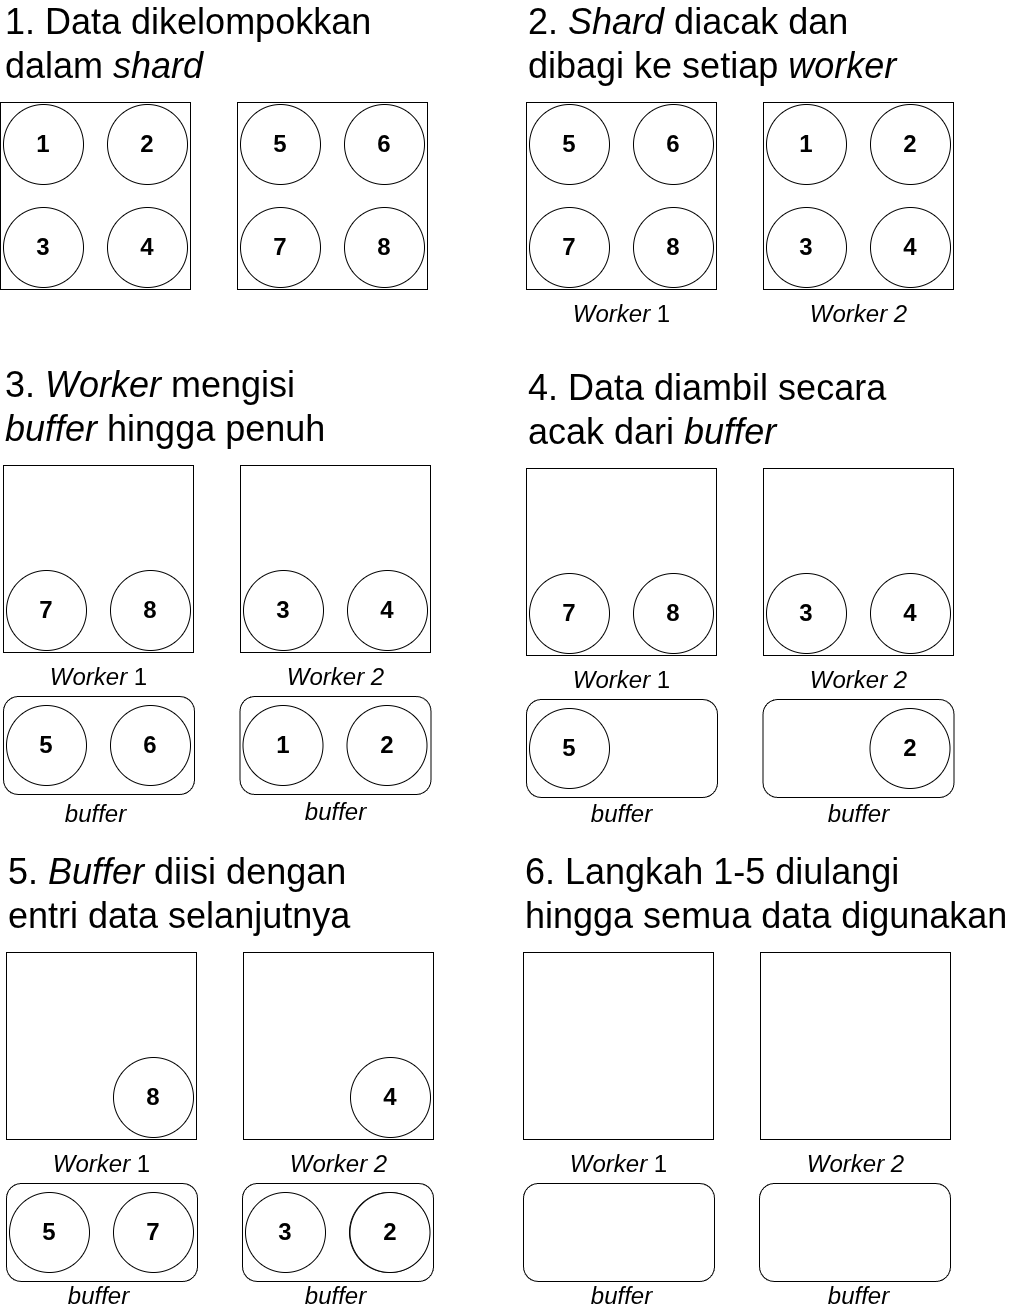
\includegraphics[width=0.7\textwidth]{BufferedShuffling.png}
    \caption{Algoritma \textit{Buffered Shuffling}}
    \label{fig:BufferedShuffling}
\end{figure}

Dua lapisan pengacakan tersebut diimplementasikan sesuai dengan Gambar \ref{fig:BufferedShuffling}. Lapisan pertama adalah pengacakan urutan \textit{shard}: pada awal setiap \textit{epoch}, urutan dari seluruh partisi (\textit{shard}) \textit{dataset} diacak terlebih dahulu. Hal ini memastikan bahwa urutan pemrosesan potongan-potongan besar data akan berbeda pada setiap \textit{epoch}. Lapisan kedua adalah pengacakan di dalam \textit{buffer}, yang bekerja dengan mekanisme yang mirip dengan \textit{reservoir sampling}. Untuk setiap \textit{worker}, sebuah \textit{buffer} dengan ukuran \textit{k} diisi dengan \textit{k} data pertama dari sebuah \textit{shard}. Ketika satu data diminta oleh proses pelatihan, sebuah data akan dipilih secara acak dari \textit{k} data di dalam \textit{buffer}. Posisi yang kosong di dalam \textit{buffer} tersebut kemudian langsung diisi oleh data berikutnya dari \textit{shard} yang sama, menjaga ukuran \textit{buffer} tetap konstan. Proses ini memastikan setiap data yang diberikan ke model merupakan sampel acak dari "jendela" data berukuran \textit{k}.

\subsubsection{Implementasi \textit{Bundle Shuffling}}
Serupa dengan strategi sebelumnya, \textit{bundle shuffling} juga diimplementasikan secara kustom melalui sebuah kelas PyTorch bernama \texttt{BundleShuffleDataset} (implementasi dari kelas ini dapat dilihat pada Lampiran X). Kelas ini mewarisi dari \texttt{torch.utils.data.Dataset} dan merujuk pada konsep dari publikasi aslinya \parencite{BundleShuffle}. Namun, dilakukan penyederhanaan pada tugas akhir ini, alih-alih menyebar logika \textit{shuffling} ke dalam tiga komponen (\texttt{Dataset}, \texttt{DataLoader}, dan \texttt{Sampler}) seperti pada implementasi rujukan, seluruh logika dikonsolidasikan ke dalam kelas \texttt{BundleShuffleDataset} untuk mempermudah implementasi.

\begin{figure}[t]
    \centering
    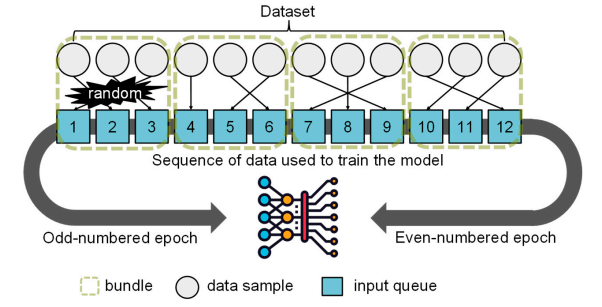
\includegraphics[width=1.0\textwidth]{BundleShuffle.png}
    \caption{Algoritma \textit{Bundle Shuffling}}
    \parencite{BundleShuffle}
    \label{fig:BundleShuffling}
\end{figure}

Mekanisme kerja algoritma ini, yang diilustrasikan pada Gambar \ref{fig:BundleShuffling}, diawali dengan tahap pra-pemrosesan. Pada tahap ini, seluruh data dalam \textit{dataset} dikelompokkan menjadi \textit{M} buah bundel, di mana setiap bundel berisi sejumlah data yang berurutan. Setelah bundel terbentuk, proses pengacakan terjadi pada setiap \textit{epoch} dengan dua karakteristik utama:
\begin{enumerate}
    \item Pengacakan Internal Bundel: Pada awal setiap \textit{epoch}, urutan data di dalam setiap bundel diacak secara individual. Ini memastikan bahwa model menerima data dalam urutan mikro yang berbeda setiap kalinya.
    \item Urutan Akses Bundel Bergantian: Yang menjadi karkateristik unik dari strategi ini adalah urutan pemrosesan bundel yang bersifat deterministik dan bergantian. Pada \textit{epoch} ganjil, bundel diakses secara berurutan dari awal hingga akhir (Bundel 1, 2, ..., \textit{M}). Sebaliknya, pada \textit{epoch} genap, urutan akses dibalik, yaitu dari akhir ke awal (Bundel \textit{M}, \textit{M-1}, \textit{M-2}, ..., 1).
\end{enumerate}

Pola akses bundel bergantian ini menciptakan ketergantungan temporal jangka panjang yang dapat diprediksi. Data-data yang berada di bundel terakhir sebuah \textit{epoch} ganjil akan menjadi data-data pertama yang diakses pada \textit{epoch} genap berikutnya (dan sebaliknya). Karakteristik ini memberikan sinyal prediktif kuat yang berpotensi untuk dieksploitasi oleh strategi \textit{prefetching} yang cerdas.

\subsection{Analisis Karakteristik I/O NFS}
Tujuan dari tahap analisis ini adalah untuk mengkarakterisasi beban kerja I/O secara kuantitatif dan kualitatif, yang dihasilkan dari proses penjalanan beban kerja pembelajaran mendalam. Dalam analisis ini, istilah "objek" merujuk pada "berkas" individual. Analisis difokuskan pada bagaimana tiga strategi \textit{shuffling} -- yaitu \textit{global shuffling}, \textit{buffered shuffling}, dan \textit{bundle shuffling} -- memengaruhi pola serta lokalitas akses (\textit{temporal} dan \textit{spatial} locality). Terdapat hipotesis bahwa setiap strategi akan menghasilkan profil lokalitas yang unik; misalnya, \textit{global shuffling} cenderung merusak lokalitas, sementara \textit{bundle shuffling} berpotensi mempertahankannya dalam cakupan \textit{bundle}. Hasil analisis ini akan menjadi landasan untuk merancang strategi \textit{caching} dan \textit{prefetching} yang lebih cerdas dan efisien di masa depan.

\textit{Temporal locality}, atau kecenderungan sebuah berkas diakses kembali dalam waktu dekat, dianalisis menggunakan metrik \textit{reuse distance}. Metrik ini didefinisikan sebagai jumlah operasi akses yang terjadi di antara dua akses beruntun terhadap berkas yang sama. Nilai \textit{reuse distance} yang kecil secara konsisten menandakan \textit{temporal} locality yang tinggi, yang berarti berkas tersebut sangat sering digunakan kembali. Analisis distribusi \textit{reuse distance} sangatlah penting -- jika distribusinya dapat diprediksi, hal ini dapat dieksploitasi. Kebijakan \textit{cache} dapat memprioritaskan berkas dengan prediksi \textit{reuse distance} terkecil, sementara \textit{prefetcher} dapat secara prediktif mengambil berkas yang diperkirakan akan segera diakses kembali.

\textit{Spatial locality}, atau kecenderungan beberapa berkas untuk diakses secara berdekatan dalam waktu, dianalisis menggunakan konsep \textit{lift}. Metrik ini mengukur kekuatan asosiasi antara dua berkas (misalnya, A dan B) dengan menghitung rasio antara probabilitas bersyarat (berkas B diakess steelah berkas A) dengan probabilitas marginal (berkas B diakses secara umum). Nilai \textit{lift} yang lebih besar dari 1 menunjukkan adanya keterkaitan antara akses yang kuat antara A dan B. Dalam konteks \textit{prefetching}, nilai \textit{lift} yang tinggi adalah sinyal jelas untuk melakukan \textit{prefetch} terhadap berkas B setelah A diakses. Selain itu, dalam konteks \textit{caching}, informasi ini dapat dimanfaatkan oleh kebijakan eviksi. Misalnya, saat berkas A diakses, \textit{cache} dapat meningkatkan prioritas berkas B yang berasosiasi kuat (jika sudah ada di \textit{cache}) agar tidak tereviksi, sebagai antisipasi atas akses yang akan datang.
